\documentclass[11pt]{article}
\usepackage{fullpage,lipsum,amsmath,amsfonts,amssymb,graphicx, subcaption,enumitem,mathtools,float}
\font\titlefont=cmr12 at 20pt
\font\subtitlefont=cmr12 at 17pt

\title{%
  \titlefont{COMS W4701: Artificial Intelligence, Spring 2025} \\
\subtitlefont{Homework \#2}} %replace \# with number
\author{Peter Driscoll (pvd2112)} %replace with name & uni

\begin{document}
\maketitle

%Problem 1
\section*{Problem 1}

\subsection*{1.1)}
By increasing the decay rate to 0.99, each iteration only reduces the temperature by $1\%$,
keeping the temperature higher for a longer period.
This favors exploration over exploitation and increases the total number of search iterations at relatively higher temperatures.
In Figure 1(a), we can see how the error count decreases more steadily over time in a single run at decay=0.99.
Meanwhile, Figure 1(b) shows that for a 30-run batch at decay=0.99,
most trials end with very few errors—indicating that the slower temperature drop helps avoid local minima.

\begin{figure}[H]
\centering
\begin{subfigure}{0.48\textwidth}
  \centering
  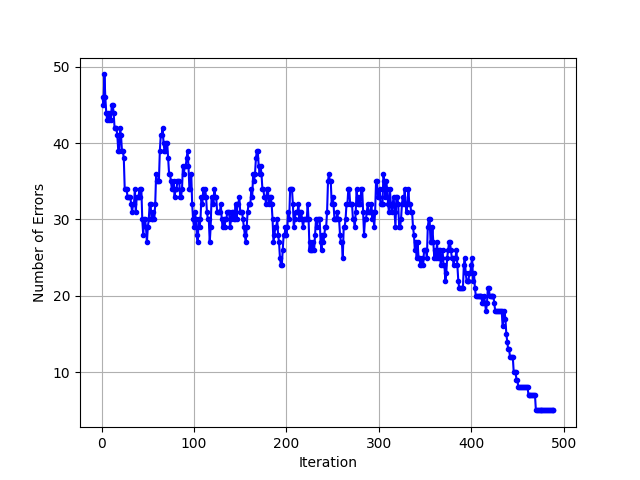
\includegraphics[width=\textwidth]{images/Figure_1.png}
  \caption{Error history of a single run}
  \label{fig:error_history}
\end{subfigure}
\hfill
\begin{subfigure}{0.48\textwidth}
  \centering
  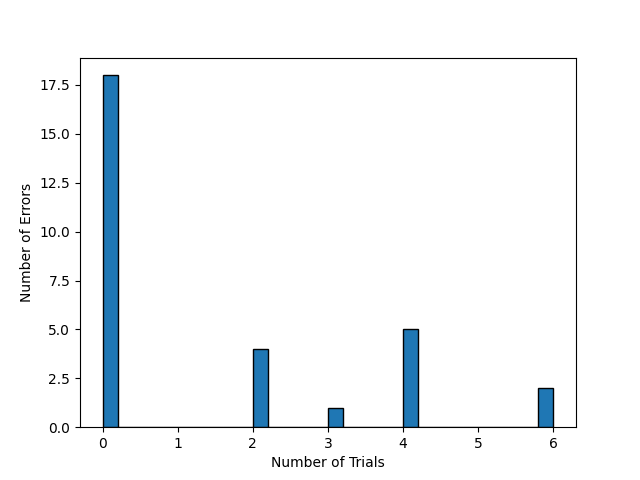
\includegraphics[width=\textwidth]{images/Figure_2.png}
  \caption{Final error histogram of 30 searches}
  \label{fig:error_histogram}
\end{subfigure}

\caption{Comparison of error tracking in simulated annealing}
\vspace{1em}
\label{fig:comparison}
\end{figure}

\begin{figure}[H]
\centering
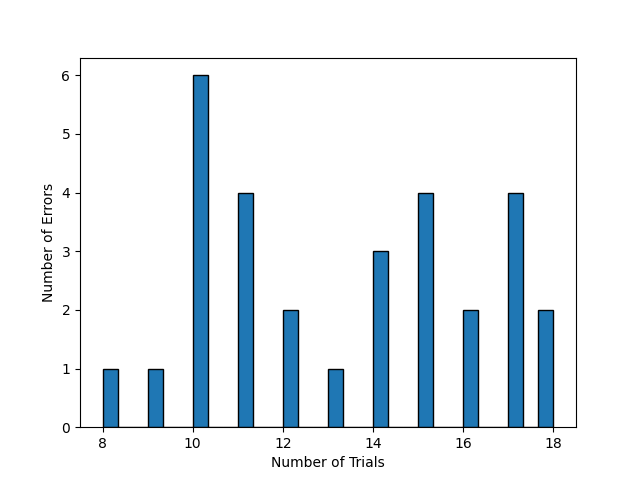
\includegraphics[width=0.8\textwidth]{images/Figure_11.png}
\caption{Cooling the decay to 0.9}
\label{fig:cooling}
\end{figure}
In contrast, for decay=0.9, the temperature decays much more quickly.
As illustrated by the histogram in Figure 2, none of the 30 trials were error-free, and fully half of them ended with 14 or more errors.
This strongly suggests that a faster drop in temperature progresses the search too quickly,
limiting its ability to accept uphill moves that might lead to better solutions later. Hence, while setting the decay=0.9 might converge more quickly,
it often converges to suboptimal states.
\newpage

\subsection*{1.2)}
The starting temperature value is inversely related to the speed of the search progression. A higher starting temperature significantly increases the variability in the number of errors early on, because the system is more willing to accept uphill moves.
Reducing the starting temperature accelerates the search, favoring exploitation, but also risks premature convergence.

For instance, when setting $T_{start} = 1$, the error count often drops quickly in the first few iterations—suggesting rapid exploitation of good moves, but then stalls out in a local minimum.
In a 30-run batch, none of these trials ended completely error-free, and half resulted in 14 or more remaining errors by the time the search stopped.

By contrast, raising $T_{start}$ to 5 or 10 introduces more early randomness,
making the error trajectory fluctuate initially but giving the search a better chance to escape bad configurations.
While this can take more iterations to produce a meaningful drop in errors, it also tends to yield fewer unsolved puzzles overall.
\begin{figure}[ht]
\centering
%--- Top row: two subfigures side by side ---%
\begin{subfigure}{0.48\textwidth}
\centering
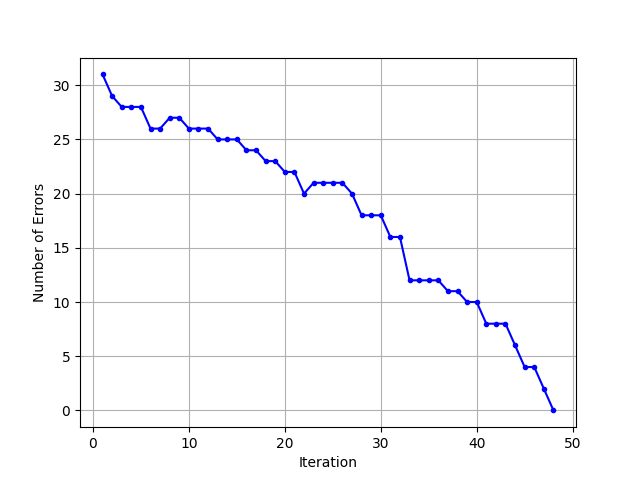
\includegraphics[width=\textwidth]{images/Figure_3.png}
\caption{Starting temperature = 1}
\label{fig:startT_1}
\end{subfigure}
\hfill
\begin{subfigure}{0.48\textwidth}
\centering
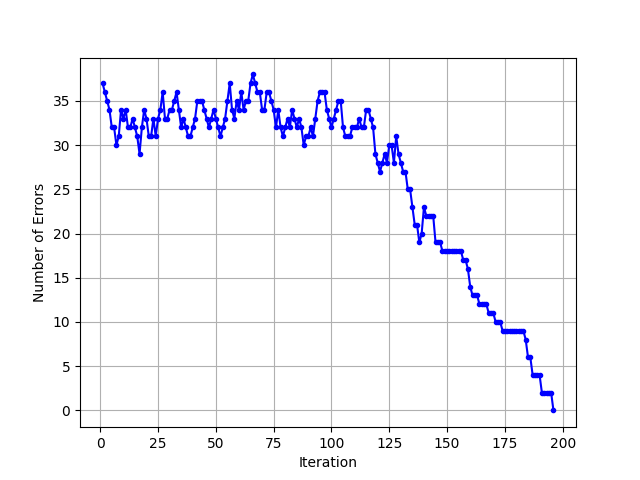
\includegraphics[width=\textwidth]{images/Figure_4.png}
\caption{Starting temperature = 5}
\label{fig:startT_5}
\end{subfigure}

%--- Add vertical space between the rows ---%
\vspace{1em}

%--- Bottom row: one subfigure (can be full width or 0.48 again) ---%
\begin{subfigure}{0.48\textwidth}
\centering
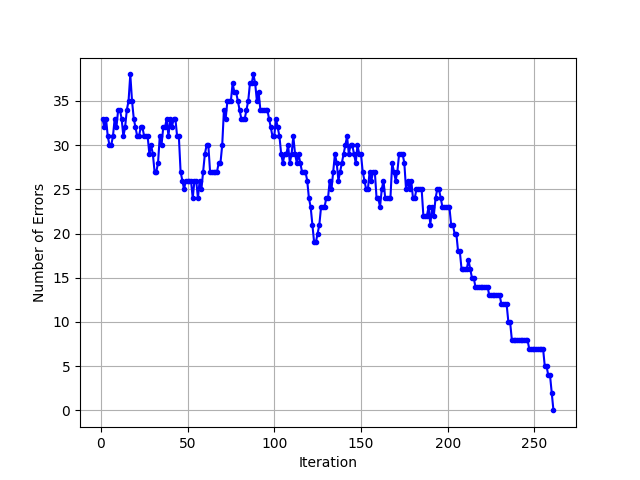
\includegraphics[width=\textwidth]{images/Figure_5.png}
\caption{Starting temperature = 10}
\label{fig:startT_10}
\end{subfigure}
\caption{Ascending values of starting temperature}
\end{figure}

\newpage

\subsection*{1.3)}
Repeating the above procedure for a batch of 30 runs at different starting temperatures $T_{start}$,
we see a clear relationship between initial exploration and final outcomes. As noted in Section~1.2,
lower values of $T_{\text{start}}$ (e.g., 1) lead to more rapid reductions in error early on,
but they also carry a higher risk of getting trapped in local minima. In fact, across 30 trials at $T_{start} = 1$,
none of the runs reached a completely error-free solution, and about half ended with 14 or more errors.

By contrast, when $T_{\text{start}}$ is raised to 5 or 10,
the algorithm accepts more uphill moves at the outset, producing greater fluctuation in the error metric but ultimately allowing the system to escape poor configurations.
Although this higher initial temperature can prolong the time it takes to see a stable drop in errors, the final solutions tend to be much better overall.
In the batch runs, $T_{\text{start}} = 10$ consistently yielded fewer remaining errors on average,
confirming that a more generous initial temperature helps avoid premature convergence, despite a somewhat slower start.

\begin{figure}[ht]
\centering
%--- Top row: two subfigures side by side ---%
\begin{subfigure}{0.48\textwidth}
\centering
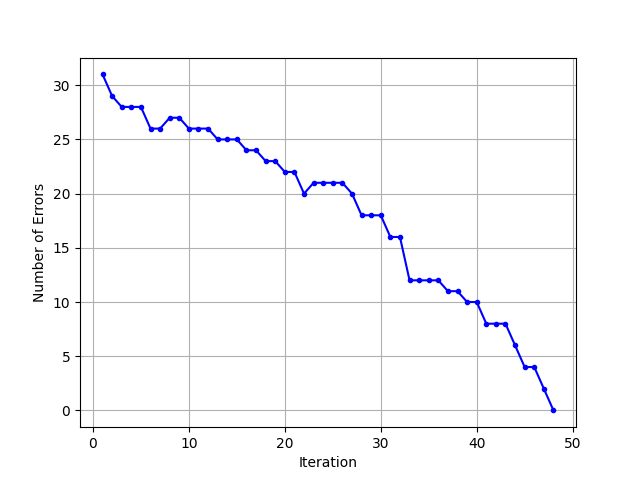
\includegraphics[width=\textwidth]{images/Figure_3.png}
\caption{Starting temperature = 1}
\label{fig:batch_startT_1}
\end{subfigure}
\hfill
\begin{subfigure}{0.48\textwidth}
\centering
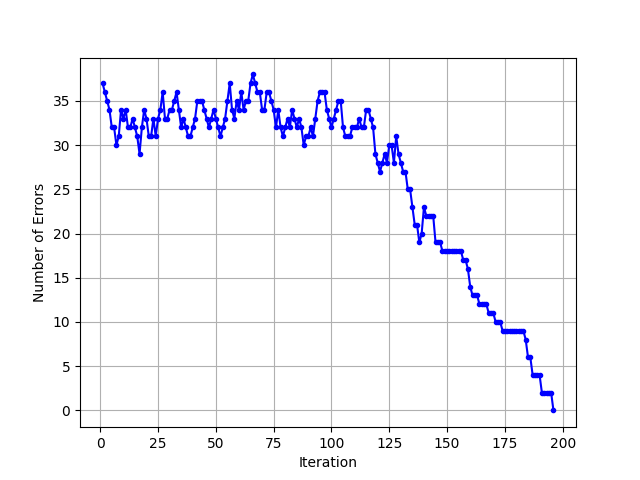
\includegraphics[width=\textwidth]{images/Figure_4.png}
\caption{Starting temperature = 5}
\label{fig:batch_startT_5}
\end{subfigure}

%--- Add vertical space between the rows ---%
\vspace{1em}

%--- Bottom row: one subfigure (can be full width or 0.48 again) ---%
\begin{subfigure}{0.48\textwidth}
\centering
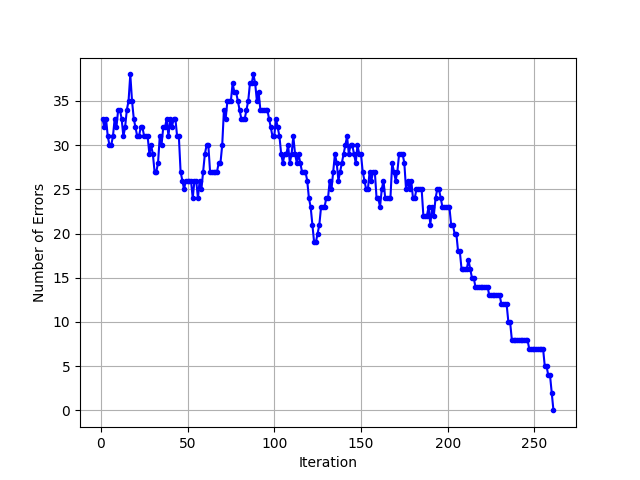
\includegraphics[width=\textwidth]{images/Figure_5.png}
\caption{Starting temperature = 10}
\label{fig:batch_startT_10}
\end{subfigure}
\caption{Ascending values of starting temperature, batch of 30}
\end{figure}

%Problem 2
\newpage
\section*{Problem 2}

\subsection*{2.1)}

\begin{center}
\begin{tabular}{lll}
$X_1 \text{ domain} = \{2,4\}$ & $X_2 \text{ domain} = \{2,4\}$ & $X_3 \text{ domain} = \{2,4\}$ \\
$X_4 \text{ domain} = \{2,3\}$ & $X_5 \text{ domain} = \{1,4\}$ & $X_6 \text{ domain} = \{2,4\}$ \\
$X_7 \text{ domain} = \{1,2\}$ & $X_8 \text{ domain} = \{2\}$ & $X_9 \text{ domain} = \{1,4\}$ \\
$X_{10} \text{ domain} = \{3,4\}$ &                                &
\end{tabular}
\end{center}

\subsection*{2.2)}
\begin{center}
\begin{tabular}{lll}
$X_1 \text{ domain} = \{2,4\}$ & $X_2 \text{ domain} = \{2,4\}$ & $X_3 \text{ domain} = \{2,4\}$ \\
$X_4 \text{ domain} = \{3\}$ & $X_5 \text{ domain} = \{1\}$ & $X_6 \text{ domain} = \{2,4\}$ \\
$X_7 \text{ domain} = \{1\}$ & $X_8 \text{ domain} = \{2\}$ & $X_9 \text{ domain} = \{4\}$ \\
$X_{10} \text{ domain} = \{4\}$ &                                &
\end{tabular}
\end{center}

\subsection*{2.3)}
Upon running arc consistency after assigning $X_1 = 2$, the domains of all the remaining variables would be pruned to one element, as follows:
\begin{center}
\begin{tabular}{lll}
$X_1 \text{ domain} = \{2\}$ & $X_2 \text{ domain} = \{4\}$ & $X_3 \text{ domain} = \{4\}$ \\
$X_4 \text{ domain} = \{3\}$ & $X_5 \text{ domain} = \{1\}$ & $X_6 \text{ domain} = \{2\}$ \\
$X_7 \text{ domain} = \{1\}$ & $X_8 \text{ domain} = \{2\}$ & $X_9 \text{ domain} = \{4\}$ \\
$X_{10} \text{ domain} = \{4\}$ &                                &
\end{tabular}
\end{center}

If we instead continued with backtracking search and assigned $X_6 = 4$, the next iteration of the search would terminate, as $X_2$ and $X_3$ would not have any elements satisfying their constraints. It would subsequently backpropogate and reassign $X_6$ = 2.

\newpage
%Problem 3
\section*{Problem 3}

\subsection*{3.1)}
The game tree, in MIN MAX convention, with expected values for all nodes, is listed in Figure 4 below. Intermediary nodes are labeled in blue, terminal nodes in black.

\begin{figure}[H]
\centering
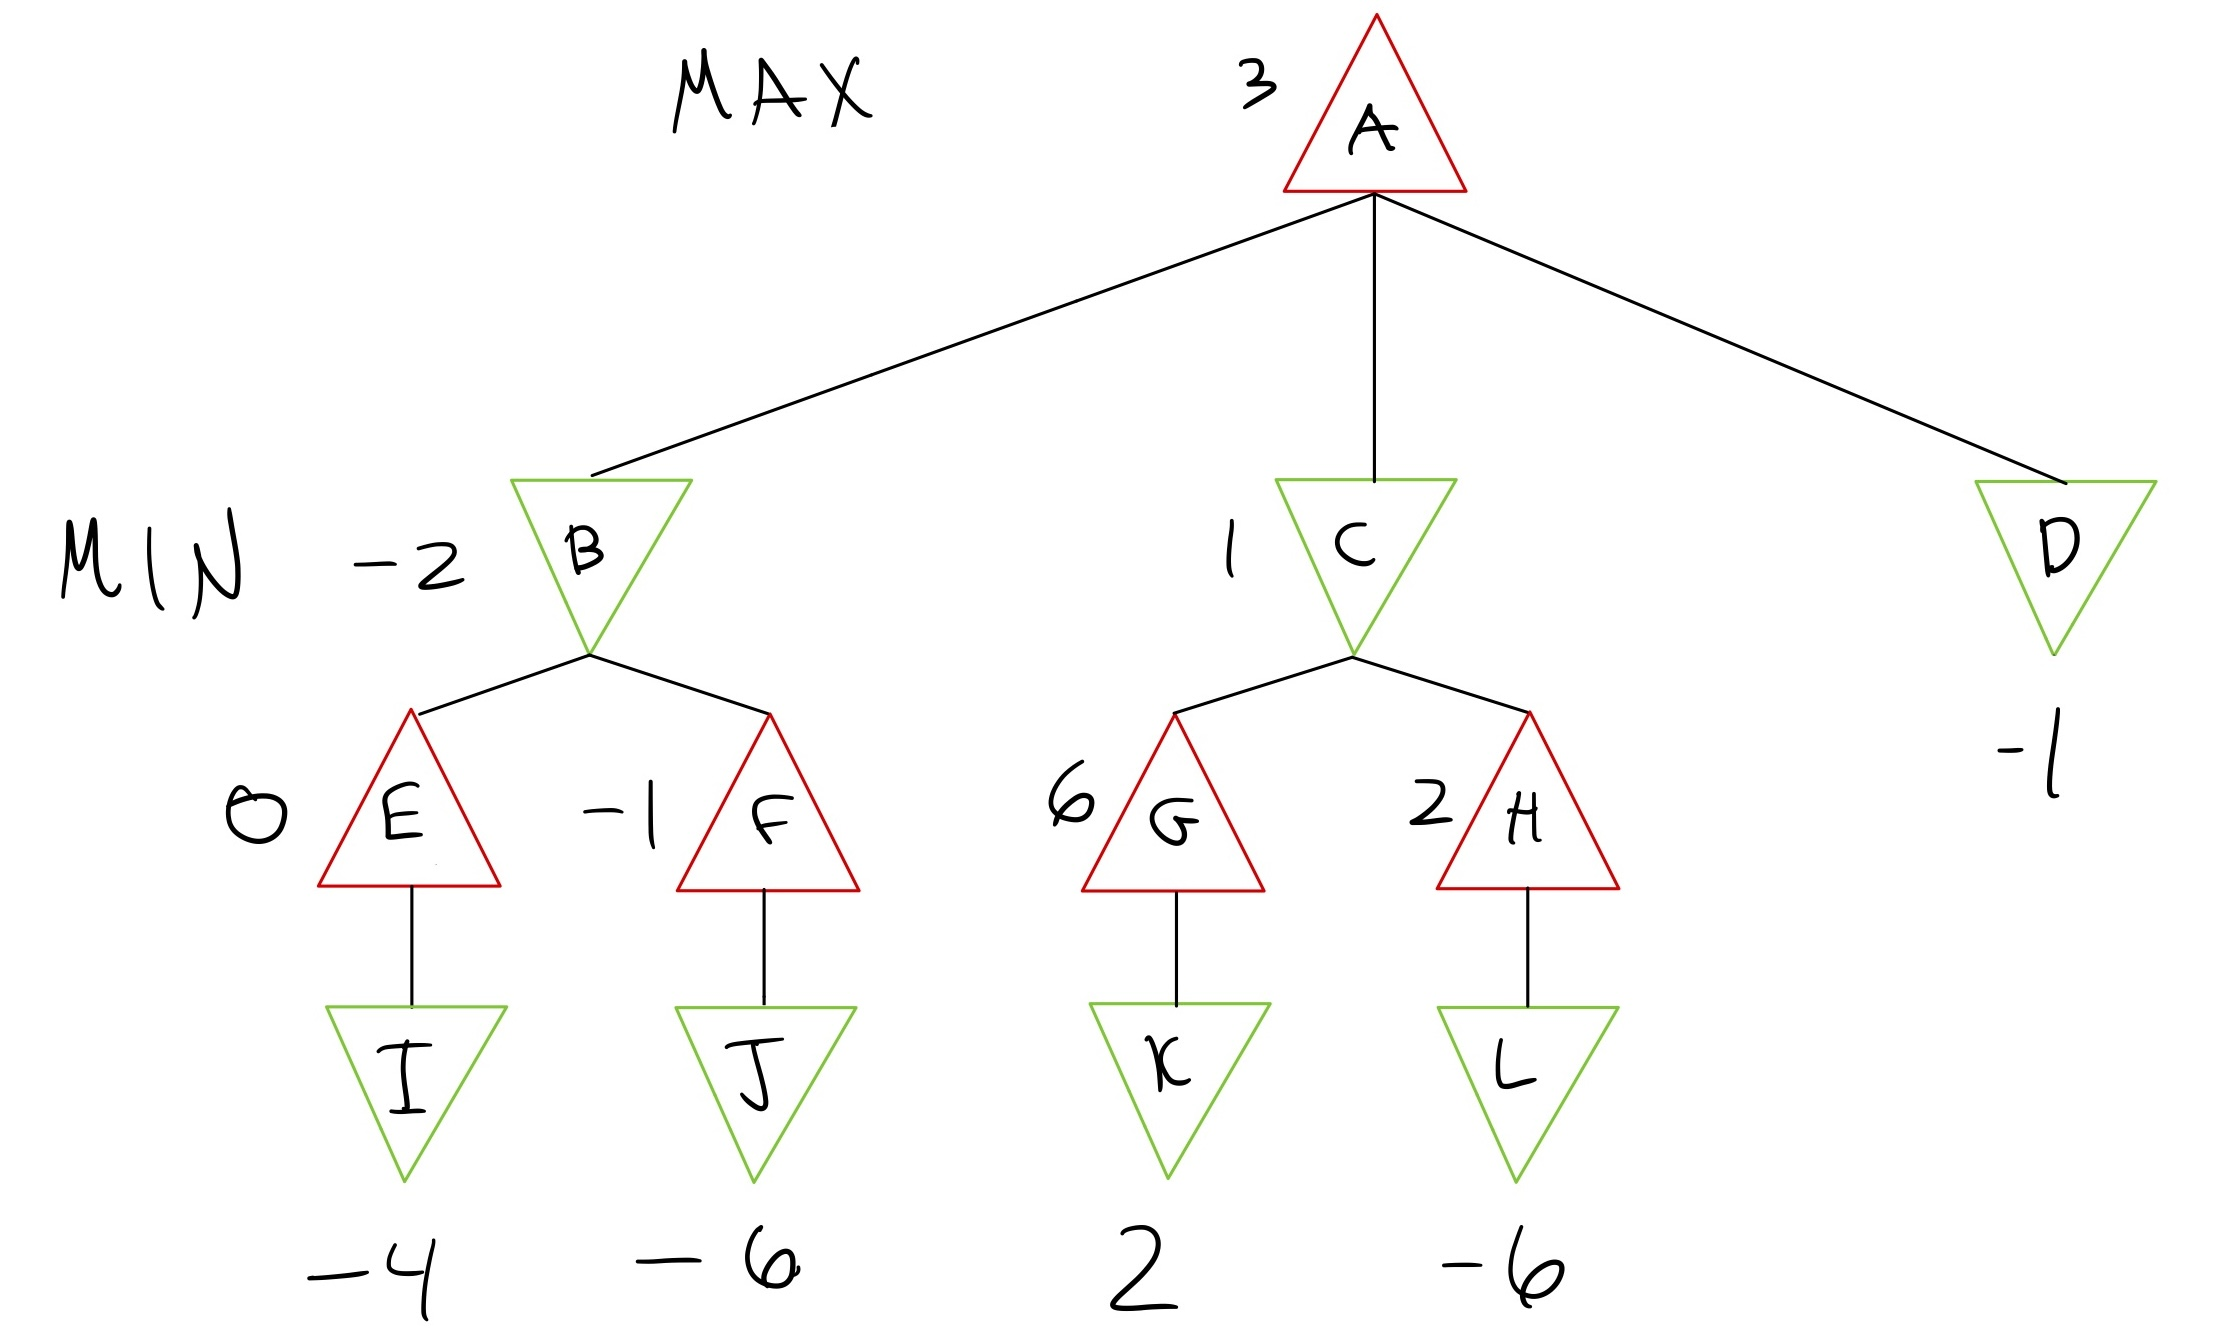
\includegraphics[width=0.7\textwidth]{images/Figure_9.jpg}
\vspace{1em}

\caption{Tic-tac-toe MAX MIN game tree}
\label{fig:game_tree}
\end{figure}

\subsection*{3.2)}
The board configurations of the leaf nodes of the game tree are listed below in Figure 6.

\begin{figure}[H]
\centering
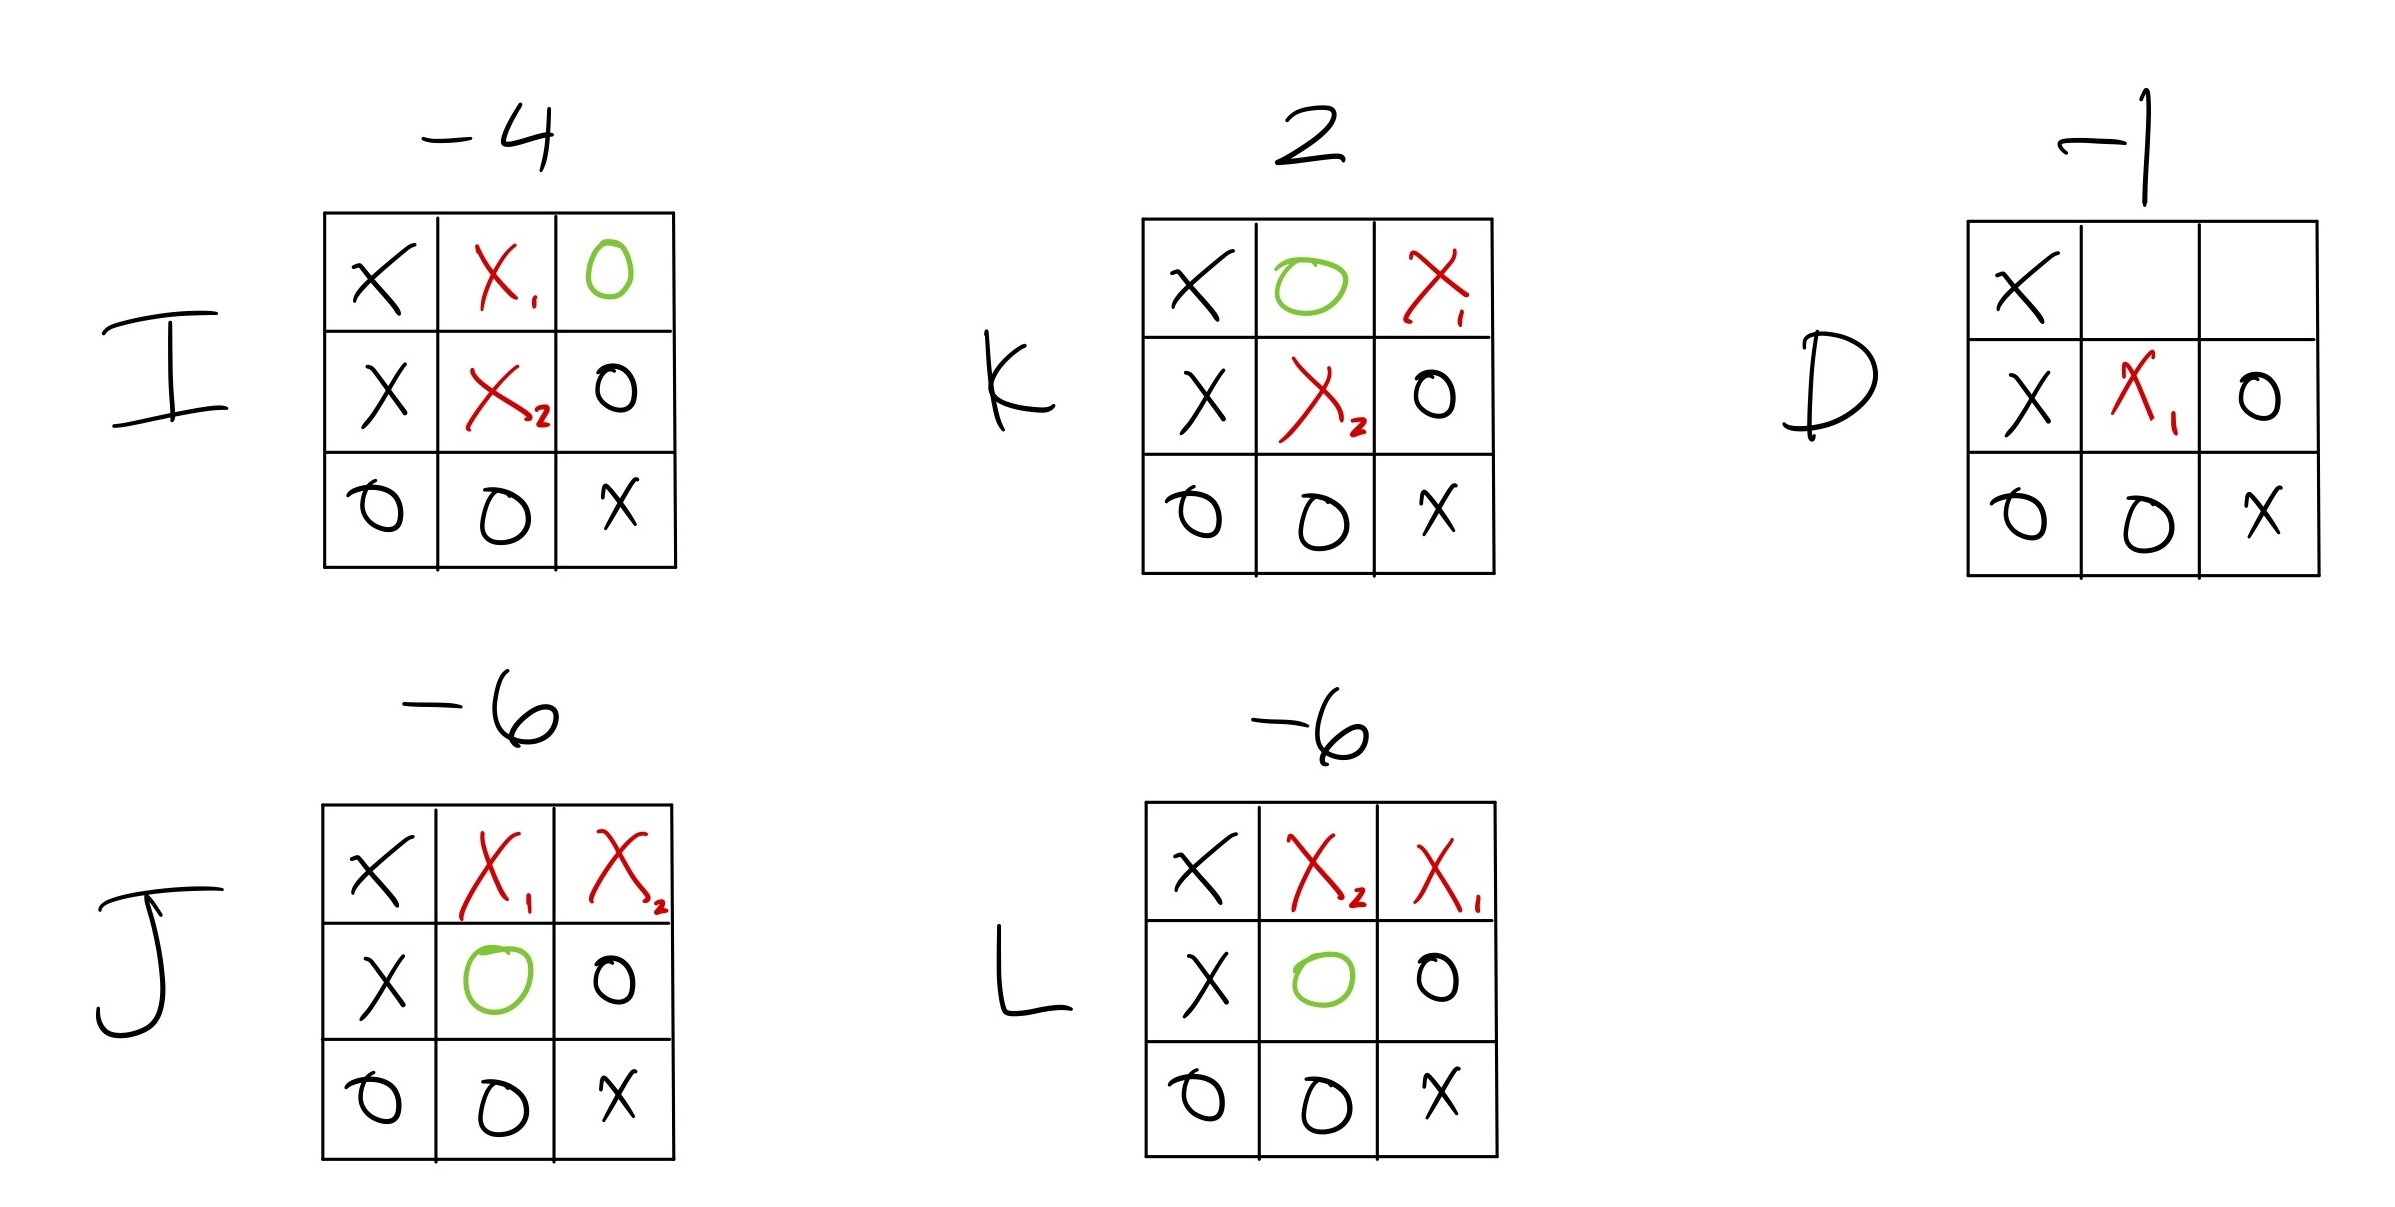
\includegraphics[width=0.7\textwidth]{images/Figure_10.jpg}
\vspace{1em}

\caption{Leaf node board configurations}
\label{fig:game_tree_leaf_nodes}
\end{figure}

\subsection*{3.3)}
\begin{flushleft}
A node sequence with no Alpha-Beta pruning: $\{A,B,E,K,F,L,C,G,M,H,N,D\}$
\end{flushleft}

\subsection*{3.4)}
\begin{flushleft}
A node sequence with maximum Alpha-Beta pruning: $\{A,D,C,G,M,B,E,K\}$
\end{flushleft}

\subsection*{3.5)}
Making O stochastic significantly impact the expected values of intermediary nodes in the game tree, thus altering X's behavior at the root.
Whereas before, the MIN nodes were certain to be the minimum of the leaf nodes, they now represent a blended average,
given by the expected values of the leaf nodes.
This gives new weight to terminal states which previously had no influence on the MIN value that was backpropogated to the MAX root node,
which increases the tree's sensitivity to unlikely states with extreme values. Furthermore, O choosing nodes based on remaining tile value
is an inverse of its expected behavior previously, as it was certain to choose terminal nodes, and consequently, intermediary nodes, which minimized the
final score of the game.
Accordingly, the optimal gameplay for X is now (1,3), with O most likely to choose (1,2), and X picking (1,1), yielding a final score of 2.
This sequence is represented as an expected value of 2/3 for the C node,
composed of the 5/6 probability O chooses node G, which yields node K with a terminal value of 2, and the 1/6 probability O chooses node H,
which terminates on node L with a value of -2.

\subsection*{3.6)}
Because the score of the game is fixed at -1 if X chooses the upper right tile,
it is straightforward to solve for the necessary probability for O in the other possible states to make X indifferent.
The expected value of the two terminal state available to O are multiplied by x and (1-x), and this sum is made equal to -1.
The following steps can be taken:
$2x -6(1-x) = -1$
$8x = 5$
$x = 5/8$.
\linebreak Thus the necessary probability to make X indifferent is 5/8 for the K leaf node and 3/8 for the L leaf node.

\newpage

%Problem 4.3
\section*{Problem 4}

\subsection*{4.3.1)}
The result of the game is 11 for p1 minimax and 5 for p2 minimax. Because minimax deterministically searches the entire game tree, this result will occur every time,
assuming the configurations of the starting board and first player to move are the same.

\subsection*{4.3.2)}
The result of playing \texttt{randy\_ai.py} against \texttt{minimax\_ai.py} is nondeterministic. Some of the results included:
minimax(p1): \{7,6,11\}, randy(p2): \{2,9,2\}. Upon swapping the order to make randy go first, some of the results included:
randy(p1): \{2,3,5\}, minimax(p2): \{14,13,11\}.
Thus, minimax clearly has an advantage over randy on the 16‐tile board. However, randy's improved competitive performance when going second
suggests that the second player is afforded a significant advantage, although randy still lost the majority of the time. Minimax playing second resulted in all
minimax wins by a significant margin. This outcome makes sense given the underlying algorithms, as minimax performs a complete search of the game tree,
finding the optimal solution, which is helped by having information about randy's first move.

\subsection*{4.3.3)}
When playing against MCTS, the only score observed with MCTS going first was a win for minimax, 11 to 2. However, when minimax was allowed to go first, this
flipped the results in MCTSs' favor, with the only score observed being MCTS 9 to minimax 3. This behavior is similarly explained by the underlying algorithm. When MCTS or minimax are
forced to go first, they have less information about the game state and have to make a less informed choice based on the generic setup of the game. This limits
the effectiveness of **each of their** search methods.

Given that the board is only 16 tiles and each player makes 8 moves in the observed games, each move
has an outsized impact on the final outcome. Although MCTS uses a probabilistic search that doesn't guarantee the optimal solution, while minimax searches the entire game tree,
the results indicate that both search methods achieve near optimality on such a small board, and the most important factor is which player goes first.

\subsection*{4.3.4)}
Upgrading to a 6 by 6 board with randy vs MCTS yielded similar results. With MCTS going second, some of the results included:
randy(p1): \{8,3,4\}, MCTS(p2): \{26,33,32\}. MCTS clearly dominates. Changing to MCTS going first, some results included:
MCTS(p1): \{29,20,19\}, randy(p2): \{6,13,12\}. Swapping the order to make MCTS go first followed a similar pattern,
with MCTS still clearly favored, though randy performed somewhat better.

\end{document}
